\section{Automatic Image Processing}

In this section we provide detailed hands-on instructions on automatic image processing within 2dx \cite{scherer20142dx_automator}, including on-the-fly image drift-correction. The here described pipeline is optimised for data recorded on a direct electron detector, such as the Gatan K2 summit. 

\subsection{Real-time motion-correction}

In case you record dose fractioned movies, we propose to drift-correct them on-the-fly as described in:

\textit{https://github.com/C-CINA/2dx/wiki/Automatic-Drift-Correction-C-CINA-setup}

Additionally instruction about setting up our automatic drift-correction pipeline is available under:

\textit{https://github.com/C-CINA/2dx/wiki/Automated-Drift-Correction-GUI}

2dx\_automator will later be used to automatically process the drift-corrected average of all frames.

\subsection{Required software}

2dx\_automator is only supported under Linux right now.
Please make sure that the list of dependencies is installed on the used system. The exact package names vary between different linux flavours. 

\begin{itemize}
	\item \texttt{TkInter} a python GUI package
	\item \texttt{py-thread} to be able to dispatch processing into different tasks
	\item \texttt{py-imaging (aka PIL)} the python image processing libraries
	\item \texttt{eman2/sparx} has to be installed and sourced on the system before launching 2dx\_automator.
	\item \texttt{py-matplotlib} to generate plots
	\item \texttt{py-shutil} for low-level operating system interactions
	\item \texttt{ImageMagic} especially the command-line tool \texttt{convert} has to be available
\end{itemize}

Additionally 2dx\_automator requires that \texttt{2dx\_image, 2dx\_merge} are available in the command line. If you installed a pre-compiled package please add 2dx's binary directory to your path:

\texttt{export PATH = /opt/2dx/bin:\$PATH}

If you compiled the software from source directly on your computer, you should source the installation-binary folder as well:

\texttt{export PATH = <your\_install\_dir>/bin:\$PATH}

where \texttt{<your\_install\_dir>} equals the second argument passed to the \texttt{build\_all}-script. If you did not pass any argument to the build-script then \texttt{<your\_install\_dir>} equals \texttt{\textasciitilde{}/2dx/}.

\subsection{Automation setup}

The basic folder organisation is shown in \autoref{fig:autoworkflow}: The raw images are stored in the \textit{raw data folder}. Note that we here only process averages gained from drift-corrected movie-frames. 2dx\_automator will check for newly added images in this folder periodically (every second). In case a new image is added, this image is processed automatically with 2dx\_image: Defocus determination, lattice estimation, unbending, automatic masking, CTF-correction and map generation. Thereby the image is imported into the currently selected 2dx-project. This project contains a merge directory and a folder storing image-directories for each automatically processed image.

\begin{figure}
	\centering
	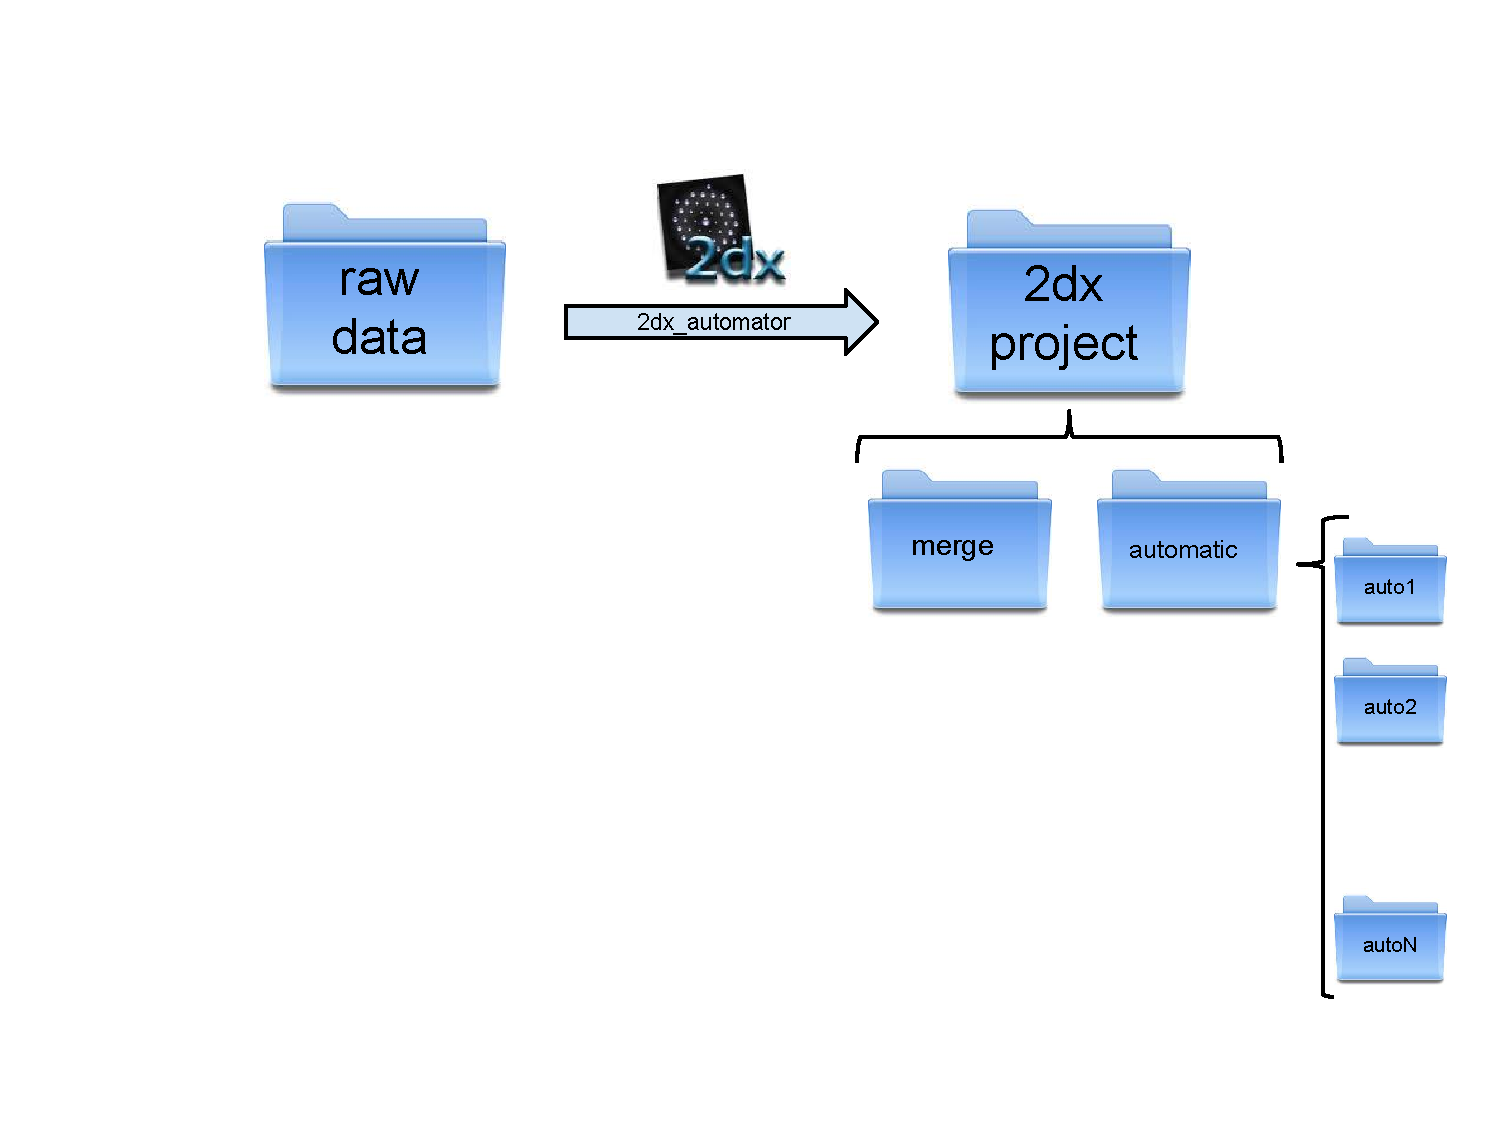
\includegraphics[width=1.0\textwidth]{auto_workflow.pdf}
	\caption{2dx\_automator: Folder structure}
	\label{fig:autoworkflow}
\end{figure}

Before launching the automation for the first time, create an empty folder, which will later contain your automatically populated 2dx-project. Then launch 2dx\_merge and select this newly generated folder as your project directory. 2dx\_merge asks whether the project structure should be generated, which should be done of course. Note that this step is only required when generating a new project. It is very important that the project structure is generated by 2dx\_merge before you launch the automation.

Starting the automation software is done by executing the command \texttt{2dx\_automator} in the shell. Given you installed all dependencies properly, 2dx\_automator will ask for two different folders. The first one you have to select is the raw images folder. Please note that you have to navigate into the folder before pressing \textit{"Ok"}. Just selecting the desired folder does not work. Secondly you are asked to select the 2dx-project. Please select the root of the project, i.e. the \textit{2dx project} in \autoref{fig:autoworkflow}.

2dx\_automator requires a config-file that stores the processing parameters used for image processing of all image. The automation software uses the file \textit{2dx\_merge.cfg} in the merge directory of the project folder (more precisely: the file linked in \textit{2dx\_master.cfg} from the root level is used). We suggest that you determine the optimal processing parameters in 2dx\_merge by manually importing and processing one or a couple of images before launching the automatic processing. Once you found the optimal processing parameters by manually processing an image in 2dx\_image you can set the tuned set of parameters as default via \textit{"File > Save as Project Default"}. Alternatively - in case you already have a valid file from a previous similar project - you can load a config file in 2dx\_automator via \textit{"Configuration > Load config from file"} directly in 2dx\_automator.

Below a couple of points to consider while tuning the image processing parameters:
\begin{itemize}
	\item Always determine the tilt-geometry (even for nominally untilted images). As 2dx\_automator does not \textit{a priori} know whether a new image is tilted or not, the processing pipeline requires these computing results.
	\item Don't use a too optimistic \textit{RESMAX} as lattice determination does get unreliable. 
\end{itemize}

Once you loaded or generated an optimal config-file, the  automatic processing is finally launched by clicking on the \textit{Launch automation} button (top-right). Note that in case there are so far unprocessed images in the input folder, these images will be processed first.

\subsection{2dx\_automator}

\begin{figure}
	\centering
	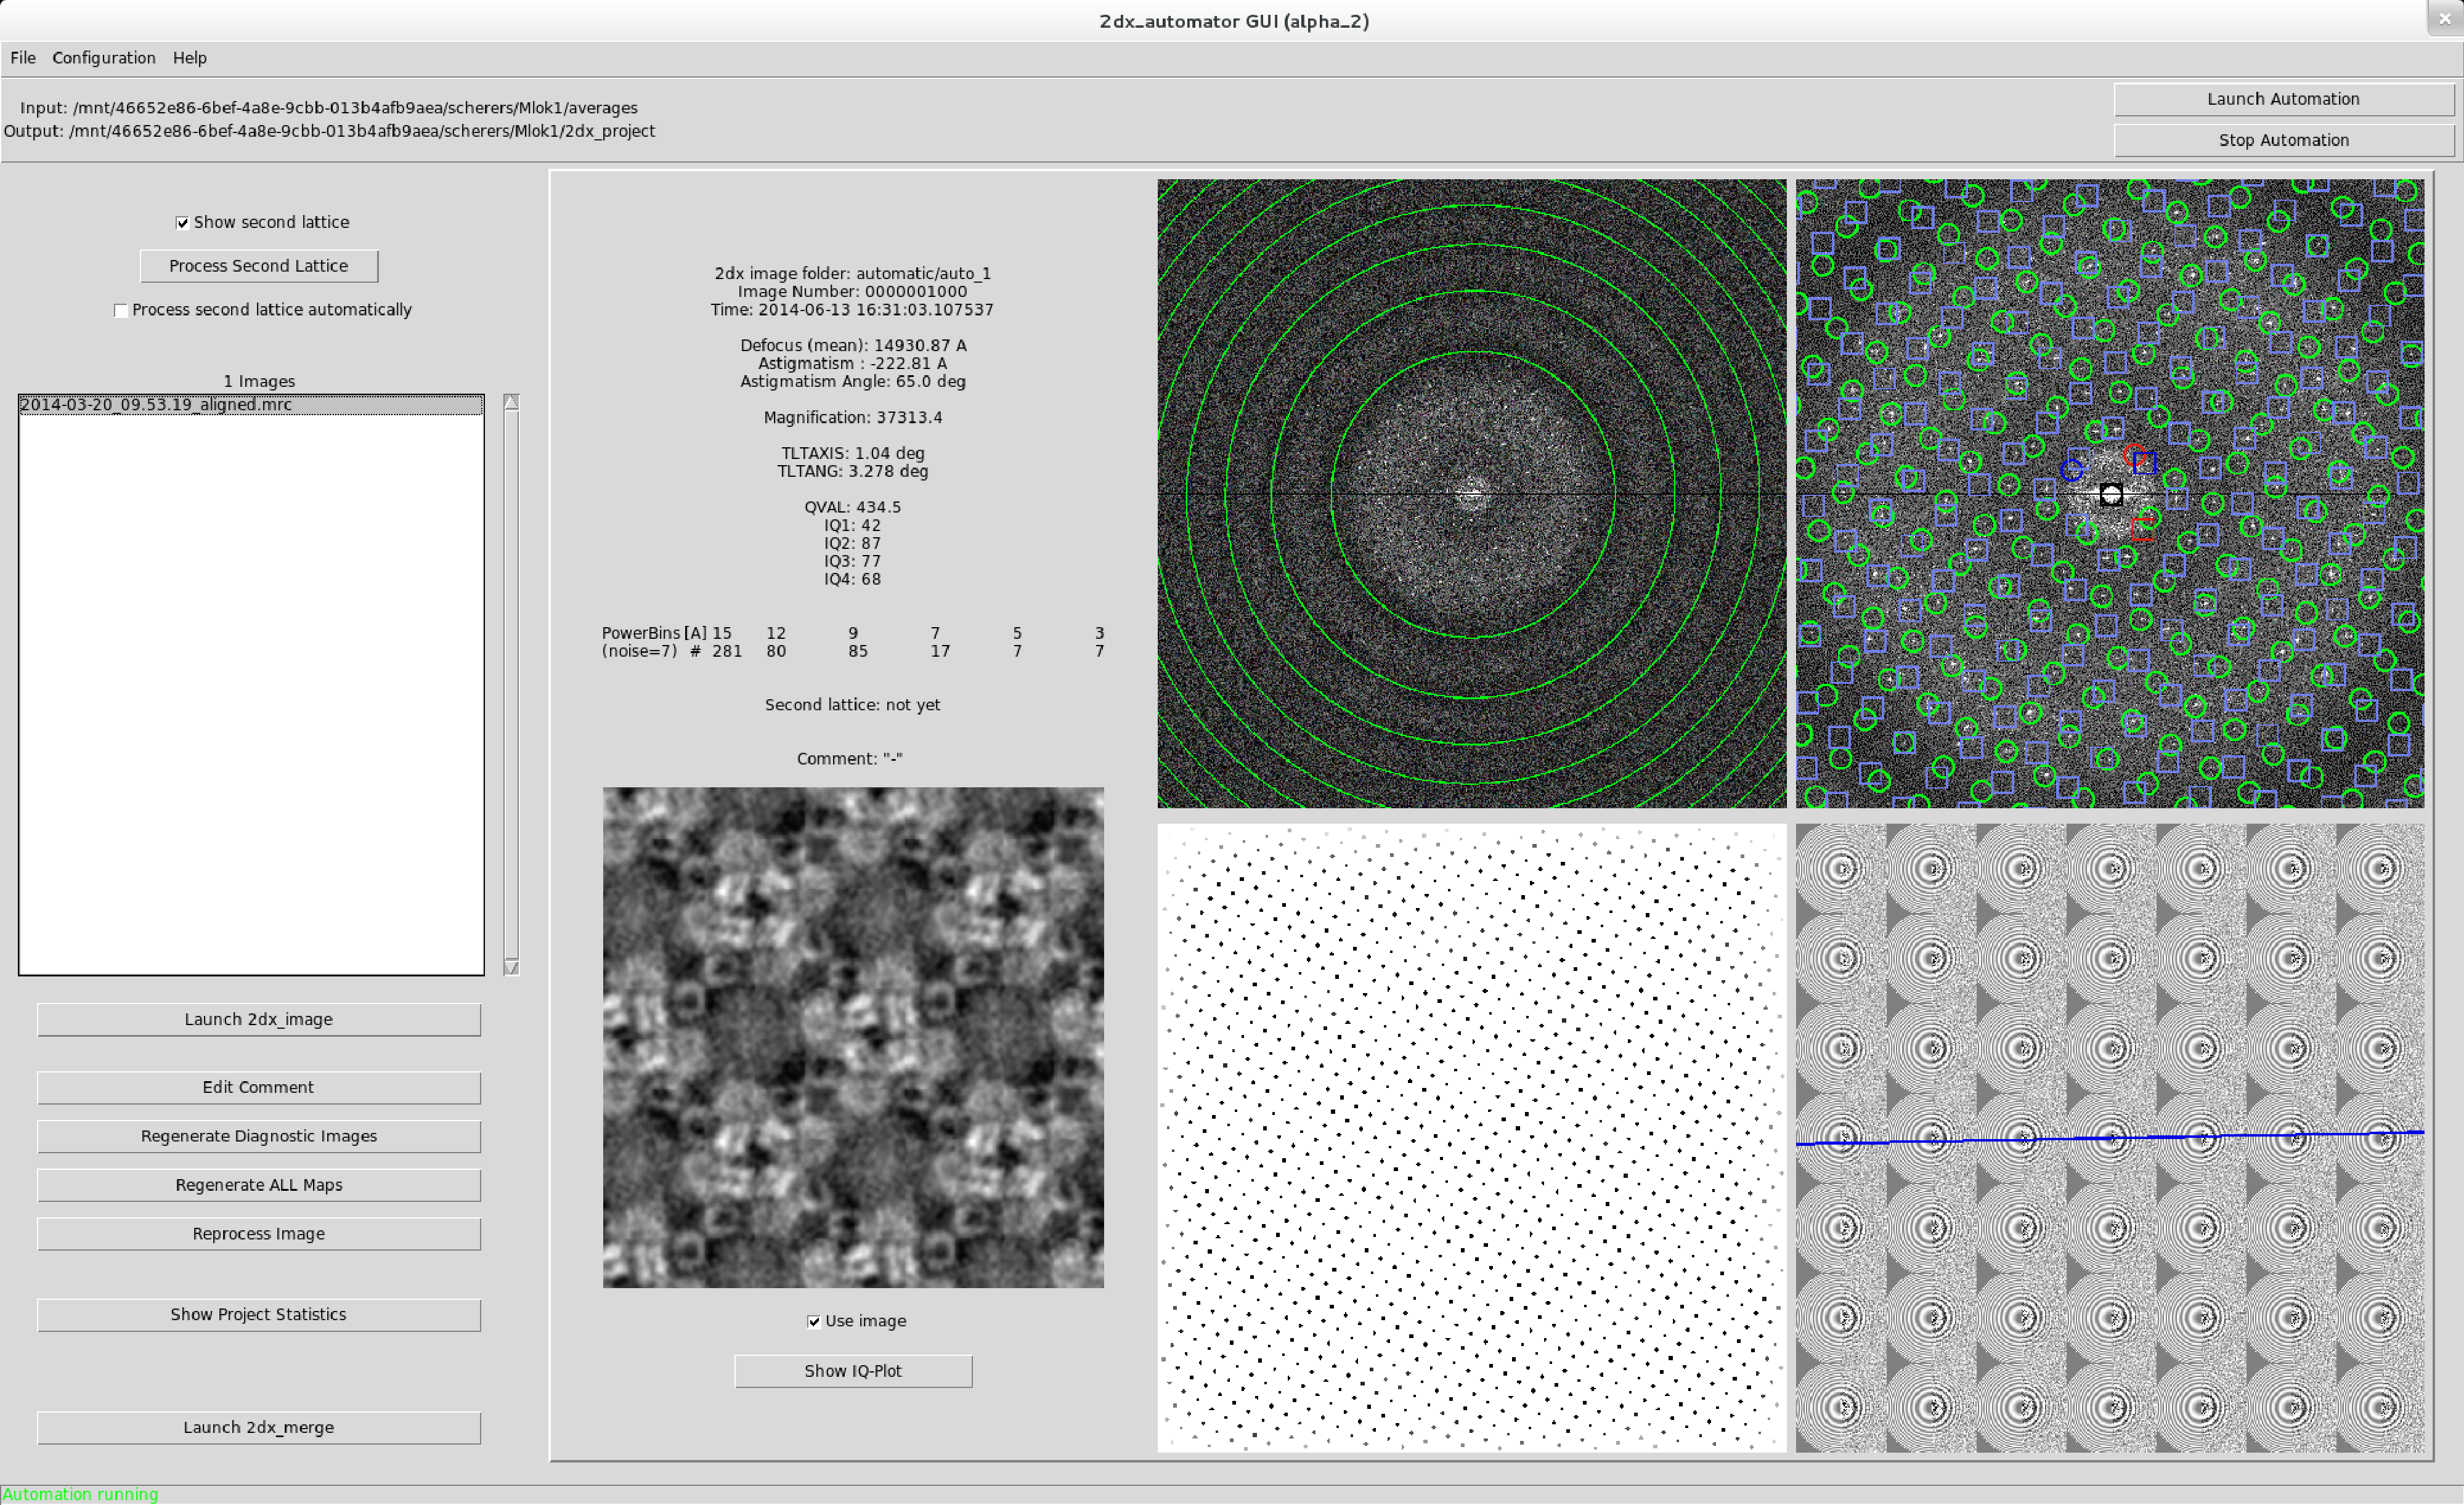
\includegraphics[width=1.0\textwidth]{auto.pdf}
	\caption{2dx\_automator graphical user interface}
	\label{fig:auto}
\end{figure}

When opening the 2dx\_automator for the first time, all fields are empty. These white squares will be populated once the images are processed, see \autoref{fig:auto}. The top row of the GUI states in which folders the automation is running and there you also can launch and stop the automatic processing, i.e. periodically checking for new images. The left panel features some processing options (detailed in \autoref{sec:auto_tricks}) and a list providing an overview of all images in the project. The right panel (detailed in \autoref{fig:auto2}) provides all required intermediate processing results, which allow to judge the reliability of the image processing of the selected image. 

In case you observe that image processing failed for one particular image, you can open 2dx\_image for the corresponding image by clicking on \textit{"Launch 2dx\_image"}. Provided you want to apply the tuned processing parameter for all future image, just save the new config parameter set as project-wide default. Once you close 2dx\_image (after fixing the processing) you have to regenerate the diagnostic images for this particular image by clicking on \textit{"Regenerate Diagnostic Images"}. Note that this can take up to 30 sec. 


\begin{figure}
	\centering
	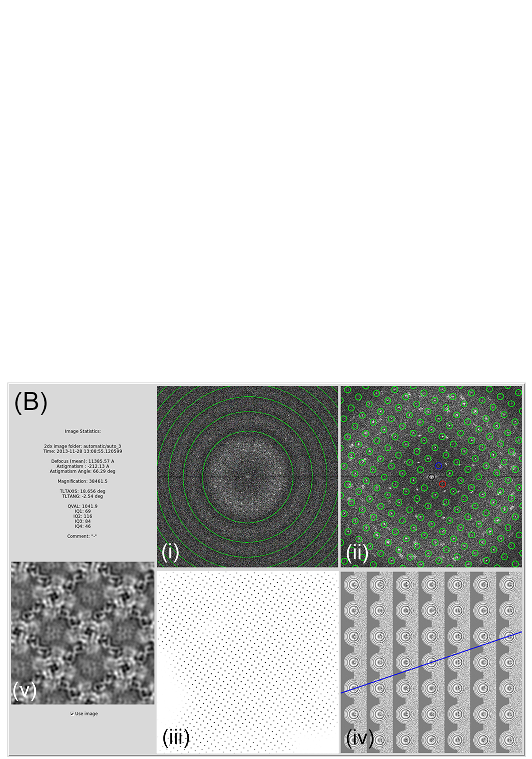
\includegraphics[width=1.0\textwidth]{auto2.pdf}
	\caption{Diagnostic view of the 2dx\_automator GUI. (i) Fourier transform with Thon rings and (ii) fitted lattice, (iii) peak profile from the unbending step used to mask the image, (iv) locally estimated defocus values, (v) final 2D projection map.}
	\label{fig:auto2}
\end{figure}


\subsection{Advanced tricks}
\label{sec:auto_tricks}

Here we discuss some advanced automation tricks, accessible via the available buttons.

\begin{description}
	\item [Second lattice processing] 2dx\_image by default tries to find two crystal lattices, given there are to (usually originating from tubular crystals). The top-left region of the central widget contains the related functions. There you can select whether the second lattice should be displayed or not. In case the second lattice was found correctly, it might be worth to processes this lattice automatically as well. Clicking on \textit{"Process Second Lattice"} clones the image directory, swaps the lattices and processes the cloned image automatically. Note that the result will not be shown in the GUI, but will be directly in the 2dx project. For instance processing the second lattice of image \textit{"auto\_12"} will generate a new image called \textit{"auto\_12\_c1"}. Enabling automatic processing of all found second lattices removes the manual selection step mentioned above. This option should be used carefully and only for high-quality datasets with clear second lattices.
	
	\item [Comment editing] 2dx\_automator provides a instant comment editing tool. You can add or edit the comment field via \textit{"Edit Comment"}. The updated comment is synchronised with the config file of the selected image.
	
	\item [Updating image maps] For instance after 3D merging it might be a good idea to regenerate the projection maps given their updated phase origins. You can regenerate all projection maps of the project by means of \textit{"Regenerate ALL Maps"}.
	
	\item [Reprocess an image] \textit{"Reprocess Image"} deletes all processing results for the selected image, copies the new config file and reprocesses the image. This function is particular useful to apply an updated config file to an image.
	
	\item [Project statistics] The judge the completeness and diversity of the recorded data, clicking on \textit{"Show Project Staticstics"} produces a project statics overview (example show in \autoref{fig:auto_stat}). Missing tilt angles are defocus values can be found efficiently by analysing the produces charts.
	
	\item [\textit{"Use images"}] Only selected images are used to generate the projection statistics overview plots.
	
	\item [IQ-Stat analysis] To judge the quality and distribution of the diffraction spots \textit{"Show IQ-Plot"} opens the \textit{PLOTRES}-file of the selected image.
	
	\item [Configuration file handling] Under \textit{Configuration > Show config file} and  \textit{Configuration > Show processing parameters} you can view the full underlying config file, respectively only the extracted processing parameters.

	\item [\textit{"Launch 2dx\_merge"}] To merge the entire project in order to get a reconstruction you have to open 2dx\_merge. Clicking on the corresponding button opens 2dx\_merge, but still asks for the desired project directory. 
\end{description}


\begin{figure}
	\centering
	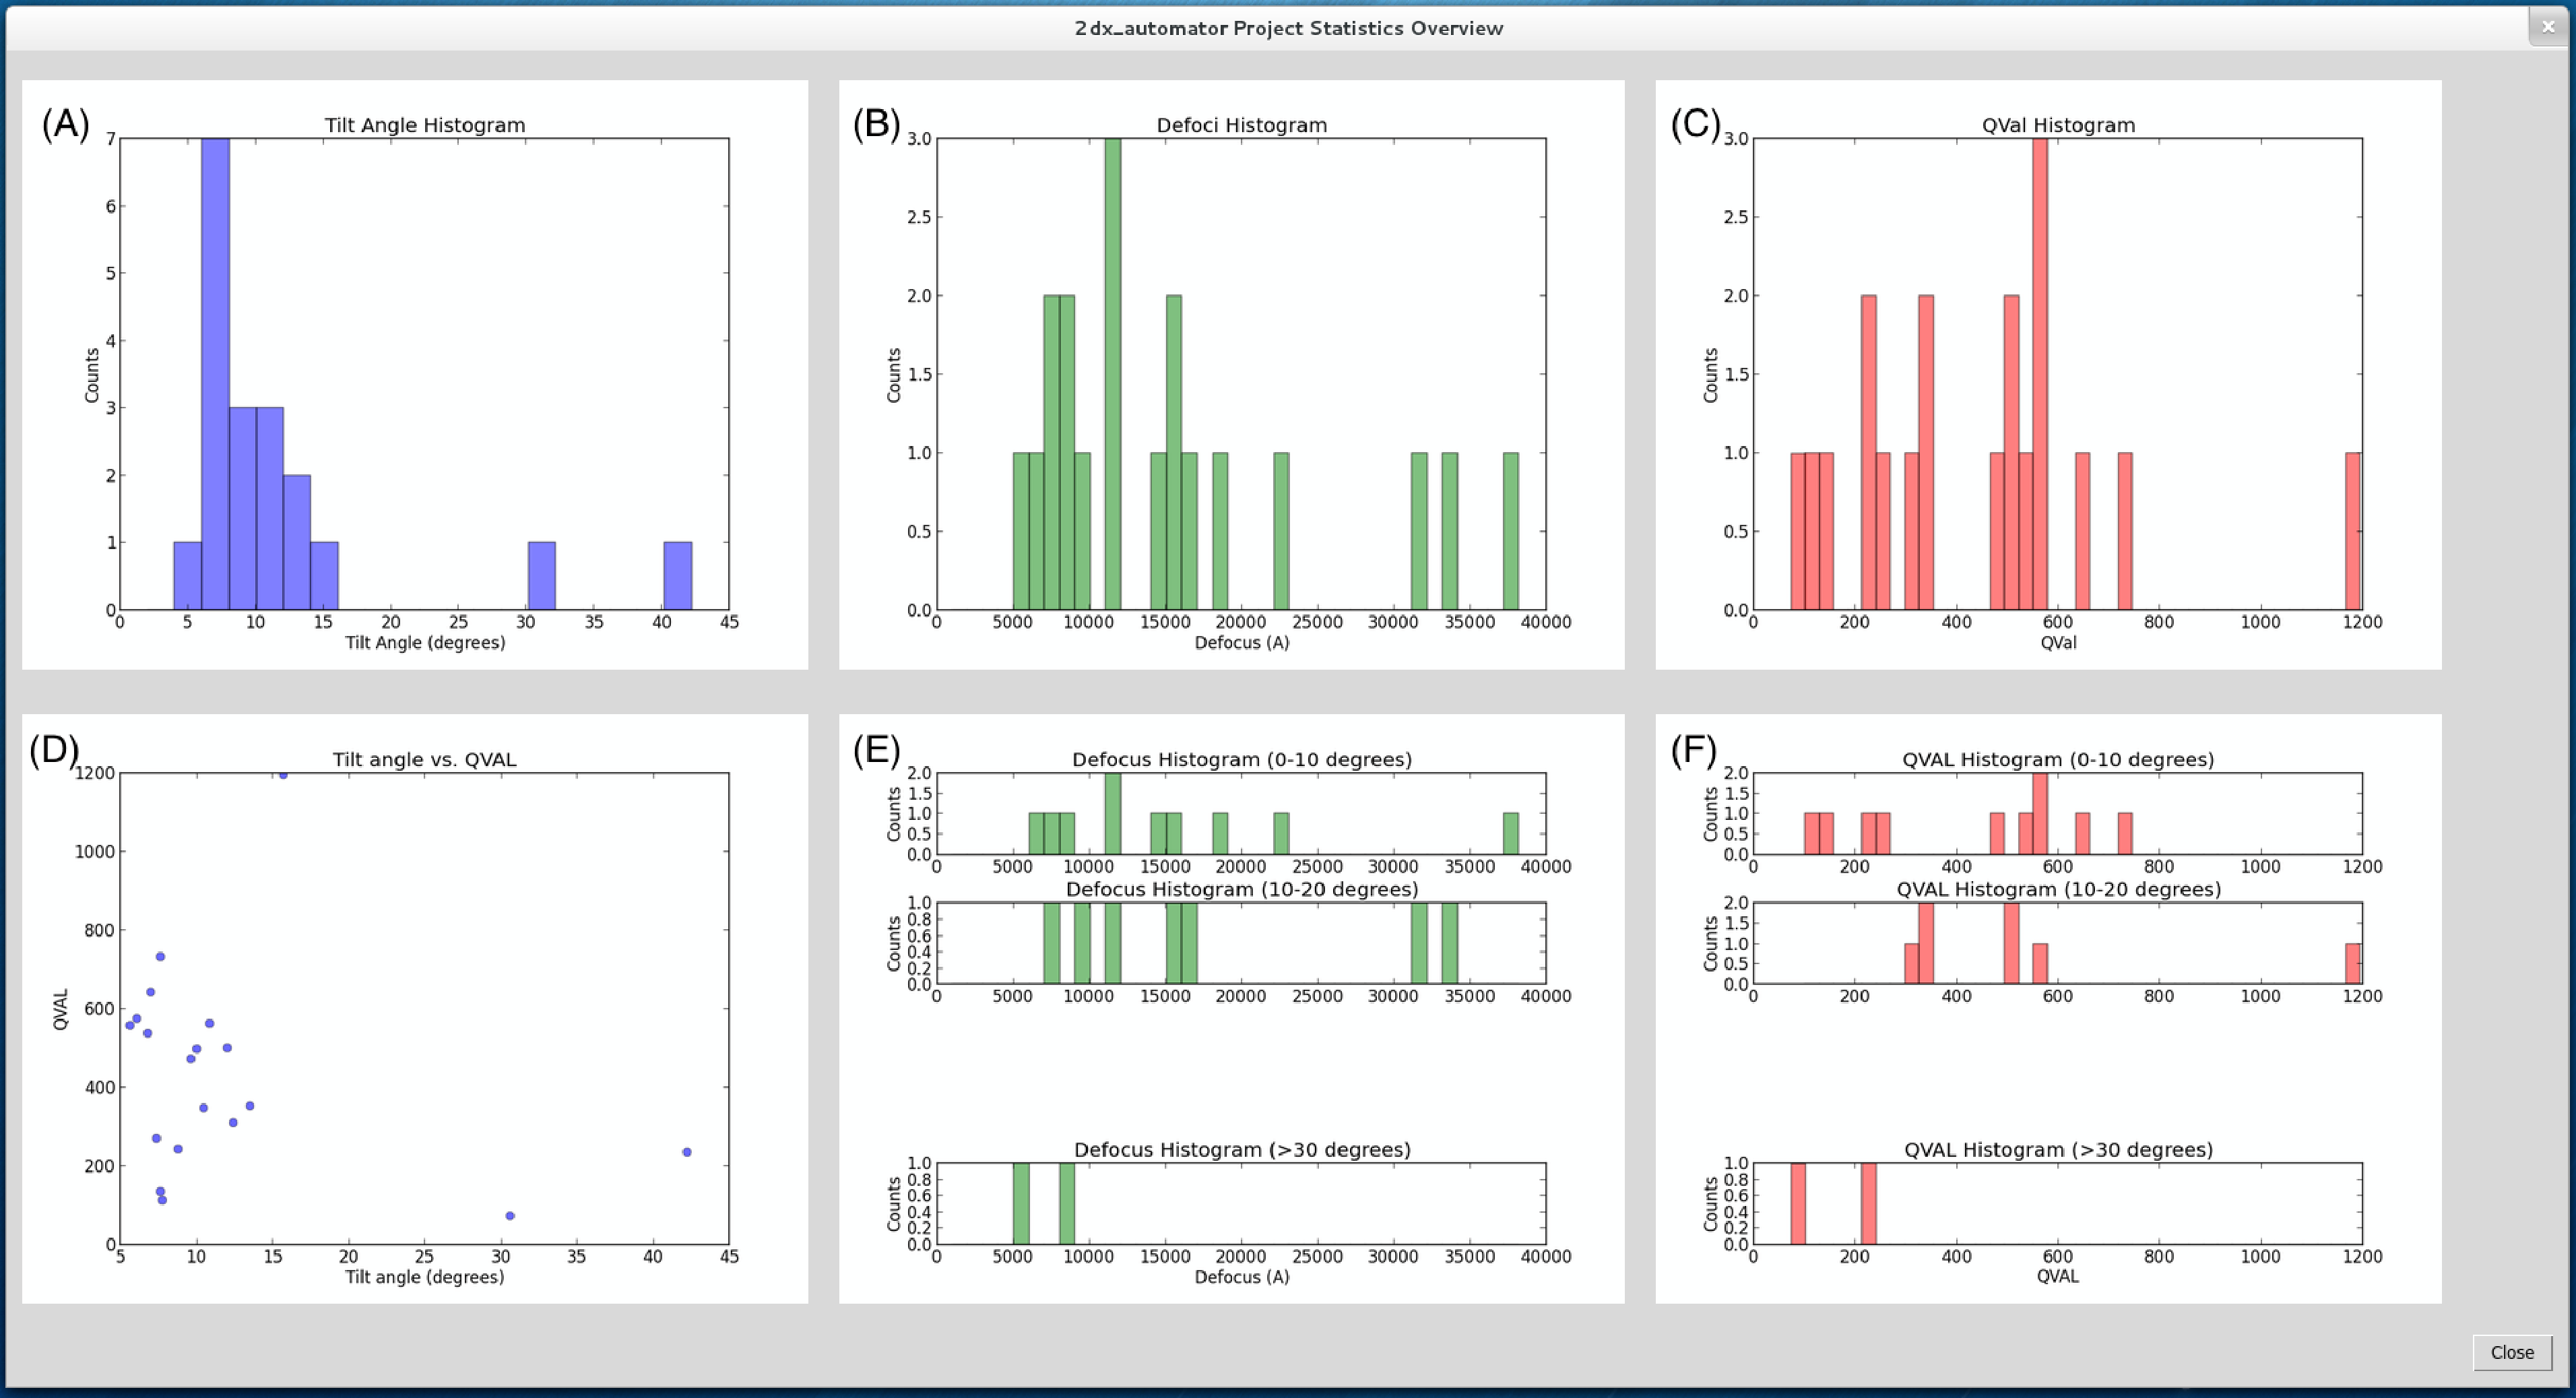
\includegraphics[width=1.0\textwidth]{auto_overview.pdf}
	\caption{Project stat}
	\label{fig:auto_stat}
\end{figure}

\subsection{Credit}
Please don't forget to cite \cite{scherer20142dx_automator} if you obtained your results by means of 2dx\_automator.